\chapter{Existing Attacks on \KECCAK}

In this chapter, we summarise the attacks on \KECCAK{}. The following are the basic types of attacks relevant to a cryptographic hash function:
\begin{enumerate}
    \item \textbf{Preimage Attacks}
    \item \textbf{Collision Attacks}
    \item \textbf{Second-Preimage Attacks}
\end{enumerate}
%Now, we will discuss these types of attack in detail.

\section{Preimage Attacks on Round-Reduced \KECCAK{}}

In a preimage attack, the attacker can derive a message from the digest of the hash function. For a $n$-bit hash value, in general, it takes $O(2^{n})$ computations to compute the message using the brute-force attack. This kind of attack is avoided by designers of hash function by setting the size of the digest accordingly. An attack with complexity greater than or equal to $O(2^{80})$ is considered computationally hard to achieve. The makers of \KECCAK{} have released several variants of the hash function \SHA-$3$ with different sizes of output hash. There are four \SHA-$3$ functions  namely \SHA3-$224$, \SHA3-$256$, \SHA3-$384$ and \SHA3-$512$ with hash length $224,\;256,\;284\;\text{and}\;512$ respectively. With these hash lengths, it is very hard to compute a preimage. Cryptographers across the world are working hard to cryptanalyse the reduced round versions of \KECCAK{} by providing practical preimage attacks for these four \SHA-$3$ hash functions. Till date, there are practical preimage attacks only for $3$ rounds of \KECCAK-$224$, $2$ rounds of \KECCAK-$256$ and $1$ round of \KECCAK-$384$, \KECCAK-$512$. There are still no practical preimage attacks for $2$ rounds of \KECCAK-$384$, \KECCAK-$512$. These preimage attacks provided by various cryptographers involve cryptanalysis of the underlying transformations per round and try to control their behavior in some way and get the values of message variables.

There are some improved preimage attacks for $2$ rounds of \KECCAK-$384$, \KECCAK-$512$ proposed by Guo \etal in ~\cite{guo2016linear} which have complexities better than brute-force attacks but are still not practical. Similarly, there are many theoretical attacks on four \SHA-$3$ functions for a different number of rounds which are better than brute-force. Improving and achieving practical preimage attacks for reduced-round variants of \KECCAK{} is an active area of research and in this thesis, we address the same.

In \cite{guo2016linear}, Guo \etal describe their techniques for preimage attacks where they use linear structures to linearize variables up to $3$ rounds. The Linear structures are the states of \KECCAK{} state which have a certain number of free linear variables, these free variables provide us with degrees of freedom which help in improving over brute-force attacks. These free variables form the linear structure. So, the higher the number of free variables the better the complexity of attack we can achieve provided the system of equations remains linear.

In this type of attack, we set message variables in the rate part in such a way that the state remains a linear structure for the number of required rounds. Here, we go forward with the message variables for (number of rounds - 1) $+$ half round, considering the state is linear structure and rest of round we go backward from the hash, and then build a system of linear equations and solve it to get the values of message variables. So, after a message is found from the hash we get the preimage successfully. This is a meet in the middle approach of attacking the system.

\section{Preimage Attacks on 2-round \KECCAK}

In this section, we will discuss some of the existing preimage attacks on $2$ rounds of round-reduced \KECCAK{} proposed in ~\cite{guo2016linear}. 
The figure~\ref{fig:linkeccakstate} used for denoting \KECCAK{} state, the numbers $x,y$ in each cell denotes the position of these lanes in the state.

\begin{figure}
    \centering
    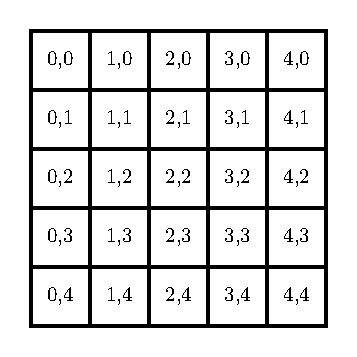
\includegraphics{keccakState.pdf}
    \caption{\KECCAK{} State with lane position specified}
    \label{fig:linkeccakstate}
\end{figure}


\subsection{Preimage Attack on 2-round \KECCAK-512}
\label{section2RKeccak512}
This attack, due to~\cite{guo2016linear}, is for $2$ rounds of \KECCAK-$512$, it uses meet in the middle approach. The first round is kept linear by linear structure and the last round, i.e.\ the second round, is inverted from the given hash value. From the given hash, they invert $\iota$ as its the simple addition of round constant for the particular round, followed by inverting only row-$0$ by the $\chi$ operation. This attack is for \KECCAK-$512$, so the hash length is $512$ i.e., $8$ lanes. Since the $\chi$ operation is like a sbox for a $row$, they invert the first row using the Observation~\ref{ob1}. So till now, we have the values of the first row of the state just before last round steps $\iota \circ \chi$. Now, Guo \etal focus on proceeding one round forward, so start with a state where lanes $(0,0), (0,1), (2,0) $ and $(2,1)$ are set as variables, rest of the part of the $rate$ is assigned random values and the $capacity$ part remains $0$ as shown in Figure~\ref{fig:2rkeccak512} where the yellow colored lanes represent variables i.e. $(0,0),\;(0,1)$ in column $0$ and $(2,0),\;(2,1)$ in column $2$. Also, the structure of the states in Figure~\ref{fig:2rkeccak512} is the same as in Figure~\ref{fig:linkeccakstate}. Lanes in white represent random values assigned to them and lanes in gray are set to all zeros in the $capacity$ part in Figure~\ref{fig:2rkeccak512}.
\begin{figure}
    \centering
    \resizebox{\linewidth}{!}{
    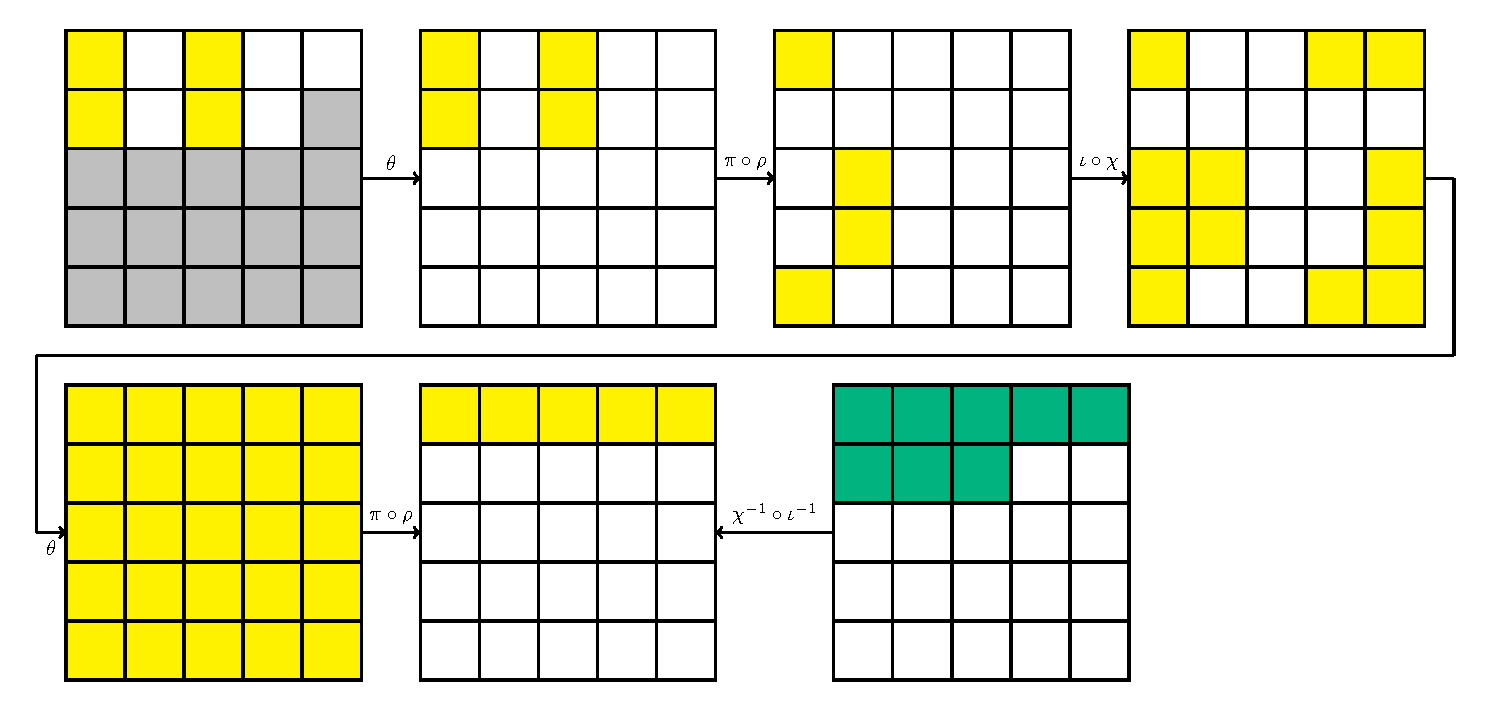
\includegraphics[scale=0.6]{2Rkeccak512.pdf}
}
    \caption{Preimage Attack on $2$-round \KECCAK-$512$}
    \label{fig:2rkeccak512}
\end{figure}
        To avoid the spreading of linear variables by $\theta$ they impose the following conditions: 
\begin{equation}
\begin{aligned}
	A[0, 1] =& A[0, 0] \oplus \alpha_{0}\\
	A[2, 1] =& A[2, 0] \oplus \alpha_{2}			
\end{aligned}
\end{equation}
        with $\alpha_0$ and $\alpha_2$ as random constants.
        
Then proceed forward with $1$st-round and the state remains linear, even after $2$nd round's $\pi \circ \rho \circ \theta$ the state remains linear since these are linear operations.
Further, build a system of linear equations from the equations of the first row of the obtained state and the values of these lanes recovered after applying $\chi^{-1} \circ \iota^{-1}$ on the hash. Then, solve the system of linear equations obtained and verify that the obtained hash is the same as the hash set for the preimage attack, if correct a preimage is found.
        
In the above method, initially there were $4$ variables lanes and after imposing $2$ conditions for the $\theta$ step, we are left with $2$ free variables each of $64$-bit namely $A[0,0]$ and $A[2, 0]$. So we observe a complexity gain over brute-force by the size of the free variables.

Hence the complexity of the attack comes out to be $2^{512 - 64 - 64} = 2^{512 - 128} = 2^{384}$. For an attack to be possible, the degrees of freedom should be greater than $512$. We have $5$ random white lanes, $2$ variable lanes, and $2$ random constants i.e. $\alpha_{0}, \alpha_{2}$, and all of these are of size $w = 64$ in our discussion. So the total degree of freedom comes out to be $ 9 \cdot 64 = 576$ which is greater than $512$ and this indicates that a solution is possible.

\subsection{Preimage Attack on 2-round \KECCAK-384}
\label{section2RKeccak384}
This attack, due to~\cite{guo2016linear} is very similar to the above attack for $2$ rounds of \KECCAK-$512$ described in section~\ref{section2RKeccak512}. We start with $6$ variable lanes with $A[0, 2] = A[0, 0] \oplus A[0, 1] \oplus \alpha_0$ and $A[2, 2] = A[2, 0] \oplus A[2, 1] \oplus \alpha_2$, where $\alpha_{0}, \alpha_{2}$ are random constants. So that $\theta$ step doesn't spread variables. We, then, proceed for the $1.5$ rounds forward and proceed backwards from the hash by applying $\chi^{-1} \circ \iota^{-1}$. Thus we set up a system of linear equations for $256$-bits and solve for message variables. Finally we check the obtained hash for correctness. Hence we observe a complexity gain over brute-force by the size of the free variables hence the complexity of the attack comes out to be $2^{384 - 4 \cdot 64} = 2^{384 - 256} = 2^{128}$. To meet the padding requirements in the worst case the complexity will be $2^{129}$.

\subsection{Practical Preimage Attack on 2-round \KECCAK-256}\label{section2RKeccak256}
    \begin{figure}
        \centering
        \resizebox{\linewidth}{!}{
        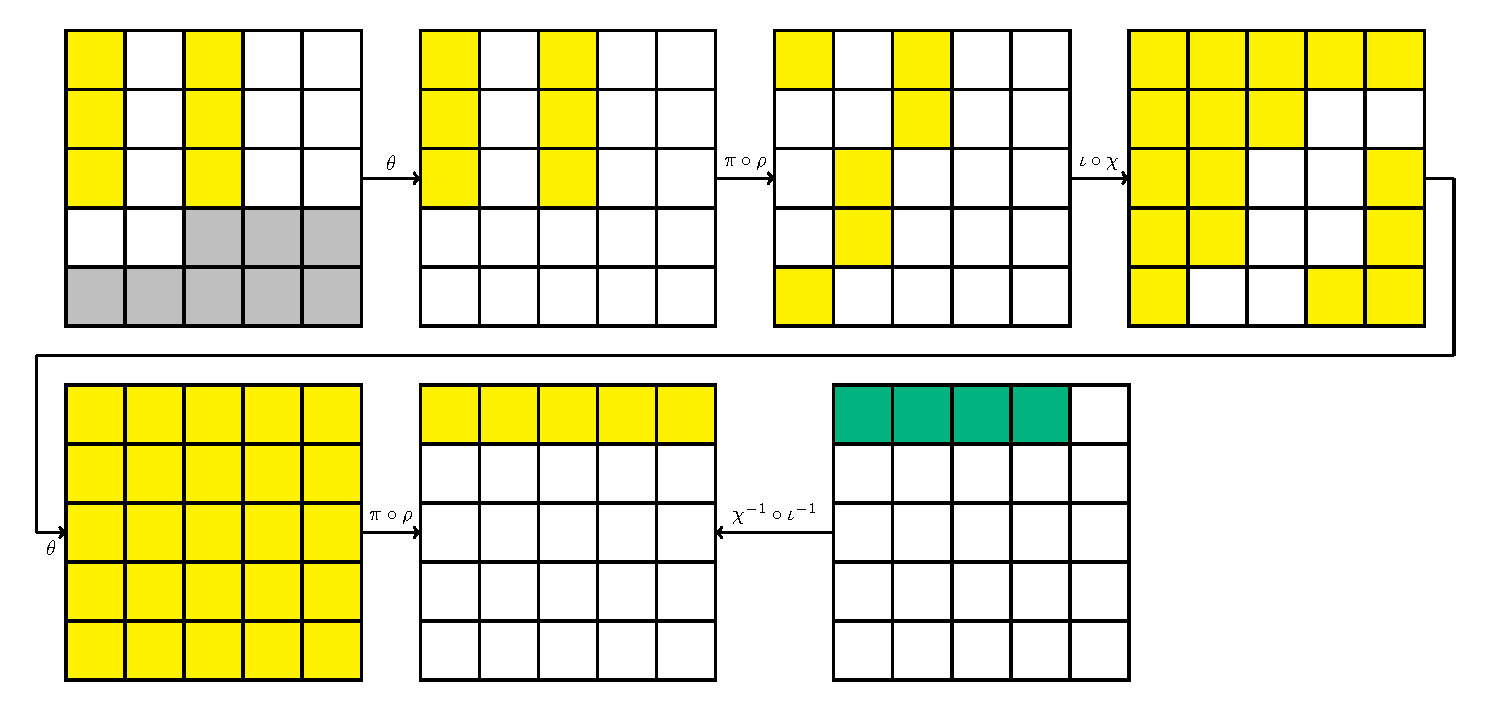
\includegraphics[scale=0.7]{2Rkeccak256.pdf}
    }
        \caption{Preimage Attack on 2-round \KECCAK-$256$}
        \label{fig:2rkeccak256}
    \end{figure}

    This attack was proposed in~\cite{guo2016linear} for $2$ rounds of \KECCAK-$256$. The attack for $2$ rounds of \KECCAK-$256$ is very similar to the attack for $2$ rounds of \KECCAK-$384$ as described in section~\ref{section2RKeccak384}. In the initial state, the message variables are in lanes $(0, 0),\;(0, 1),\;(0, 2),\;(2, 0),\;(2, 1),\;(2, 2)$, rest all lanes in rate part can take any random value as shown in Figure~\ref{fig:2rkeccak256}. We keep the sum of variables in columns $0$ and $2$ constant by choosing the sum of variables in these columns to be $\alpha_0$ and $\alpha_2$ respectively, where $\alpha_0, \alpha_2$ are random constants. Due to these conditions, the parity of columns $0, 2$ is constant and $\theta$ step would affect the full state only by a constant value.
    
    For \KECCAK-$256$, length of digest is $d = 256 \rightarrow 4$ lanes and capacity $c = 512 \rightarrow 8$ lanes. We can get $4$ linear equations on the input bits of $\chi$ given $4$ output bits out of the $5$-bits using the Observation~\ref{ob3}. Therefore, we need $4$ variables in our state to build a linear system of $256$-bit equation. We have $h_0, h_1, h_2, h_3$  hash lanes in the output. By using the property of $\chi$, we can get $4$ linear equations on the input to the $\chi$ when $4$ output bits are given. The above is true for each lane in row $0$. i.e. we can get $4 \cdot 64$ linear equations on the input state to the $\chi$ step.
    
    So, we build the initial state such that we have $4 \cdot 64$ free variables. Take $A[0, 0] = A[0, 1] \oplus A[0, 2] \oplus \alpha_0$ and $A[2, 0] = A[2, 1] \oplus A[2, 2] \oplus \alpha_2$. The state remains linear after $1$ round and half-round i.e. $\pi \circ \rho \circ \theta$, initially there were $6$ variable lanes and after imposing $2$ conditions for $\theta$, we are left with $4$ free variables each of $64$-bit namely $A[0,1], A[0,2], A[2,1], A[2,2]$ i.e. the linear structure. We observe a complexity gain over brute-force by size of linear structure, hence the time complexity of attack$\;= 2^{256 - 256} = 2^{0} = 1$.
    
    By solving the system of linear equations we get a solution in constant time. Though earlier in $2011$ a practical attack was proposed in~\cite{naya2011practical} but of complexity, $2^{33}$ and by the method of linear-structures Guo \etal in~\cite{guo2016linear} were able to compute the preimage in constant time.

\section{Preimage Attacks on 3-round \KECCAK{}}

In this section, we will discuss some of the existing preimage attacks proposed in~\cite{guo2016linear} on $3$ rounds of round-reduced \KECCAK{}.

\subsection{Preimage Attacks on 3-round \KECCAK-384, \KECCAK-512}
\label{3rkeccak512attack}
The 3 rounds of \KECCAK{} can be summarized as:
   \begin{equation}\label{3r_eq}
    M \xrightarrow[\text{1.5 rounds}]{ \pi \circ \rho \circ \theta \circ R} A \xrightarrow[]{ \iota \circ \chi } B \xrightarrow[]{ \theta } C \xrightarrow[]{ \pi \circ \rho } | \xleftarrow[]{ \chi^{-1} \circ \iota^{-1} } h  
    \end{equation}

  For $3$ rounds of \KECCAK-$512$, Guo \etal extend their attack on $2$ rounds of \KECCAK-$512$, as described in section~\ref{section2RKeccak512}. In the initial state there are $4$ variable lanes but after first $\theta$ only $2$ variable lanes are left so that the effect of $\theta$ is constant. So, we have only $128$ free variables. Then $\pi \circ \rho$ just permutate the variable lanes and after $\chi$ step the number of linear terms increases. So after the first round, almost all columns have at least one variable lane (except the 3rd column as shown in Figure~\ref{fig:2rkeccak512} ). Due to this, after $\theta$ step of the second round, the full state becomes linear and the $\pi \circ \rho$ further don't introduce any non-linear term, they only change the positions of lanes and rotate them, so the state is still linear.  These are the first $1.5$ rounds of \KECCAK{} where $0.5$ round includes only the first three step mappings i.e $\theta, \rho, \pi$. Hence the state after $1.5$ rounds i.e. $A$ remains linear.
  
  Following this is the $\chi$ of the second round since the input to $\chi$ contains linear terms and as we know $\chi$ is a non-linear operation so the output state after $\chi$ is a non-linear i.e. quadratic state. Dealing with non-linear terms is not easy, so the idea is to linearize the quadratic terms and try to reduce the complexity as compared to a brute-force attack.

  So, the bits input to step $\chi$ of the second round are all linear. We can directly invert the first 320 bits through $\chi^{-1}$ from the given hash value of $8$ lanes. Of the inverted state, each bit is a sum of $11$ bits (due to $\theta$ step) of the output of the second round though they will be permuted by $\rho, \pi$.

  Based on Equation~\ref{3r_eq}, we can express $C[x][y][z]$ in terms of $B[x][y][z]$, where  
\begin{equation}\label{Cexpression}
 C[x][y][z] = B[x][y][z] \oplus \oplus_{y' = 0}^{4} B[x-1][y'][z] \oplus \oplus_{y' = 0}^{4} B[x+1][y'][z-1]
\end{equation}
  Open all the expressions in Equation~\ref{Cexpression} and separate two terms $B[x][y][z]$ and $B[x-1][y][z]$ and the rest of the $9$ terms remain as it is.
    So we can further say that, 
        \[ B[x][y][z] \oplus B[x-1][y][z] = (a \oplus c + b) \oplus d
    \]
    where,
         \[
        a = A[x][y][z], b = A[x + 1][y][z], c = A[x + 2][y][z], d = A[x - 1][y][z]
    \]
    So guessing $b$ and other $9$ terms in Equation~\ref{Cexpression} would make $C[x][y][z]$ linear. Hence, we linearize $C[x][y][z]$ by guessing $10$ bits input to step $\chi$. These $10$ terms include $A[x + 1][y][z],\;B[x + 1][\cdot][z-1]$ and $B[x-1][y'][z]$, where $0 \leq y' \leq 4 \text{ and } y' \neq y$. Hence, we obtain $1 + 10$ linear equations, by these linear equations we can match the hash value bit corresponding to $C[x][y][z]$. So $11$ linear equations for $1$ bit of hash value. For $3$ rounds of $\KECCAK$-$512$ we have only $128$ variable bits, so we can match $128/11 = 11$ bits of the hash value.
    
    Time complexity of preimage attack $= 2^{512 - 11} = 2^{501}$.

    \textbf{Note:} There is an improvement for the above attack and is described in section~\ref{improvedkeccak512} by which attack complexity comes out to be $2^{482}$.

	The same attack can also be applied for attacking $3$ rounds of \KECCAK-$384$, where we have $4$ variable lanes as described in section~\ref{section2RKeccak384}. The $4$ variable lanes are $A[0,1],\; A[0,2],\; A[2,1],\; A[2,2]$ but we need to set the last bit of $A[2,2]$ to $1$ to satisfy padding rule. Hence we are left with $4 \cdot 64 - 1 = 255$ variable bits.
    
    Number of matched hash bits $ = 255/11 = 23 $. Time complexity of preimage attack for $3$ rounds of \KECCAK-$384$ is $ 2^{384 - 23} = 2^{361}$.

\subsection{Improved Preimage Attacks on 3-round \KECCAK-384, \KECCAK-512}
\label{improvedkeccak512}

    The idea for improvements of the attacks described in section~\ref{3rkeccak512attack} was proposed in~\cite{guo2016linear}. As explained in section~\ref{3rkeccak512attack} the non-linear term $C[x][y][z]$ is linearized by guessing $10$ bits. In this attack, Guo \etal assumed that the guessing was independent, which can be dependent too if chosen properly. So the idea is to guess for those bits which would help in reducing the number of guesses for some other bit(s). So it will be possible to reduce the complexity further by choosing linearly dependent bits so that there can be more matched bits of the hash value.

    We start with the following two equations, $B$ represents the state after $\chi$ of $1$st round as shown in the Equation~\ref{3r_eq}. Here,
        \[
            B[x][y][z] = A[x][y][z] \oplus (A[x+1][y][z] \oplus 1) \cdot A[x+2][y][z]
        \] and
        \[
            B[x-1][y][z] = A[x-1][y][z] \oplus (A[x][y][z] \oplus 1) \cdot A[x+1][y][z]
        \]
        By guessing $A[x+1][y][z]$ we make both of the above equations linear. Hence we guess terms $A[x+1][y'][z]$ where $0 \leq y' \leq 4$. Due to this, the non-linear terms $B[x][\cdot][z]$ and $B[x-1][\cdot][z]$ are linearized.
        
        Similarly to linearize $B[x+1][.][z-1], B[x+2][.][z-1]$ we guess $A[x+3][y'][z-1]$ where $0 \leq y' \leq 4$.
        
        The expression for $C[x][y][z]$ in terms of state $B$ is,        
        \[
        C[x][y][z] = B[x][y][z] \oplus \oplus_{y' = 0}^{4} B[x-1][y'][z] \oplus \oplus_{y' = 0}^{4} B[x+1][y'][z-1]
    \] and the expression for term $C[x+1][y+1][z]$ is 
        \[
        C[x+1][y+1][z] = B[x+1][y+1][z] \oplus \oplus_{y' = 0}^{4} B[x][y'][z] \oplus \oplus_{y' = 0}^{4} B[x+2][y'][z-1]
    \]
    
        These $10$ bits guessed linearize the term $C[x][y][z]$, also the term $C[x+1][y+1][z]$ after these $10$ guesses contains only one non-linear term i.e. $B[x+1][y+1][z]$. After guessing the term $B[x+1][y+1][z]$, $C[x+1][y+1][z]$ is also linearized. We can match $2$ bits by setting up $13$ ($10 + 1 + 2$) linear equations. Similarly Guo \etal set up $8$ more linear equations by guessing $6$ more bits and match $2$ more bits of hash value. So, in general if there are $t$ variables then we can match upto $ 2\floor*{\frac{t-5}{8}}$ bits of hash.

        Hence for $3$ rounds of \KECCAK-$384$ and \KECCAK-$512$, the number of variables are $255$ and $128$ respectively, which gives $62$ and $30$ matched bits.
        
        Therefore the complexities of the improved attacks are $2^{384 - 62} = 2^{322}$ and $2^{512 - 30} = 2^{482}$ respectively.

\section{Practical Preimage Attack For 2 rounds of \KECCAK-256}

Earlier in $2011$, Naya-Plasencia \etal proposed various attacks in~\cite{naya2011practical}. One of them was a practical preimage attack on $2$ rounds of \KECCAK-$256$ with an attack complexity of $2^{33}$. This attack uses meet in the middle approach, where the initial state contains $10$ lane variables in the message where each column contains $2$ variables. To avoid any effect of $\theta$, they keep the effect of $\theta$ step constant by adding constraints such that the parity of each column is $0$ which means one of the variables in the column is the same as the other. Further after applying $\pi \circ \rho$ we obtain $state2$, this state is used to build solutions in such a way that it matches the hash value. In the hash state, there are $4$ lanes and to invert complete row by $\chi^{-1}$, they assume the fifth lane in the hash state and then apply $\chi^{-1} \circ \iota^{-1}$ on the full row using Observation~\ref{ob2}. Computing further backwards apply $\rho^{-1} \circ \pi^{-1}$ to get the state (say $state3$) where only $5$ lanes are completely known. Now using the information of these $5$ lanes they find the values of the $5$ variable lanes of the message.

After applying constraints to keep $\theta$ on the message state as identity,  only $5$ variable lanes are left, i.e. $5 \cdot 64$ degrees of freedom which is the same as the number of lanes after inverting from the hash value. So it is expected to find a solution.

So, $state2$ on applying $\theta \circ \iota \circ \chi$ gives $state3$. In this method instead of directly computing the values of all message variables corresponding to the hash value they build solutions for smaller groups. 

For \KECCAK-$256$ we consider lane size $w = 64$, we start with building all possible solutions for some groups of $3$ slices of $state2$ and checking that these solutions match the values of $state3$. This required generating all possible solutions for the message variables in these $3$ slices and then discarding those solutions which don't satisfy the constraints.

Further, the solutions of the groups of $3$-slices are merged to give solutions for groups of $6$-slices and in this process we get the value of the $1$st slice of the second group because it depends on the last slice of the previous group in $\theta$ step. Further pruning of the solutions is done based on constraints due to the repetitions of variables amongst these $6$-slices.

Similarly, solutions of $12$-slices are built from $6$-slices, then in the next step solutions for $24$-slices are built. Lastly, we build solutions for $48$-slices by merging $2$ groups of $24$ slices.
 
So we have all possible solutions for the first $48$-slices by this method and we have to compute the solutions for the remaining $16$-slices.

The solutions for the remaining $16$-slices are found in a similar way where these $16$ slices are further divided into groups of $4$ and $12$ slices. The solutions for $4$ slices are found in the same way as for $3$ slices and the solutions for the $12$ slices are built in the same way as explained previously. Then solutions for both these groups are merged to get all possible for the last $16$ slices.

Moving further we merge the solutions of $48$ and $16$ slices groups and after matching the values from the $state3$ and the repeated variables we get the solution for $64$ slices and this gives the values of the $5$ message variables.

This attack has time as well as space complexity, due to the size of the solution list for a group of slices. None of the steps described above exceed $2^{31}$ time complexity. To match the padding conditions for the message further $2^2$ iterations are required in the worst case. So a preimage for $2$ rounds of \KECCAK-$256$ is practically found in $2^{33}$ time complexity and $2^{29}$ memory complexity.

\section{Collision Attacks on \KECCAK{}}

A collision attack on cryptographic hash function means that the attack is able to generate two different input messages $M_1, M_2$ to the hash function $h(.)$ such that, hash of both the messages is same i.e. $h(M_1) = h(M_2)$.

In general, we can obtain a collision attack by generating random messages and obtaining their hashes and storing this hash in a table. While storing the hash in the table if the same hash already exists then we have found a collision, otherwise, we store it in the table. This is also known as the birthday attack. If the output of the hash function is a $n$-bit hash, then the birthday attack yields a collision in $2^{n/2}$ computations of the hash function.

There are 4 different \SHA-$3$ functions namely \SHA3-$224$, \SHA3-$256$, \SHA3-$384$ and \SHA3-$512$. \SHA3-$d$ hash function in general outputs a $d$-bit hash, so the generic complexity for collision attack for \SHA3-$d$ is $2^{d/2}$.

But for \KECCAK{}, there is also another kind of brute-force attack possible. In \KECCAK{} even if there is a collision in the capacity part of the hash state then also it is possible to yield a collision attack. Let's assume we have two messages $a, b$ such that they produce the following output and $f$ is our hash-function:
\[
    f(a) \rightarrow \left[ \alpha || c \right]
\]
\[
    f(b) \rightarrow \left[ \beta || c \right]
\]
Note that the two inputs above are such that they have a collision in $capacity$ part of the output state, next we see how we can generate an actual collision from this.

Here, $M_1 = a || 0$, where the first message block consists of $a$ and second block is $0$, then
\[
    f(M_1) \rightarrow f\left( \left[ \alpha \oplus 0 || c \right] \right) \rightarrow f\left( \left[ \alpha || c \right] \right) \rightarrow S_1
\]
Let $M_2 = b || \beta \oplus \alpha$, where the first message block consists of $b$ and second block is $\beta \oplus \alpha$, 
\[
    f(M_2) \rightarrow f\left( f(b) \oplus \beta \oplus \alpha \right) \rightarrow f\left( \beta \oplus \beta \oplus \alpha || c \right) \rightarrow f\left( \left[\alpha || c\right] \right) \rightarrow S_1
\]
Both $M_1, M_2$ yield same state $S_1$ after applying hash function $f$, so a collision is found. But this method depends on the collision in the $capacity$ part of the state which requires $2^{c/2}$ computations of the hash function by birthday attack. So the actual complexity for the collision attack of \KECCAK{} hash function with a hash of size $d$-bits and capacity of $c$ bits is $min\left( 2^{c/2}, 2^{d/2}\right)$.

\KECCAK{} didn't observed much collision attacks before the year $2011$. In the year $2011$, the first practical collision attack on $2$ rounds of round reduced \KECCAK-$256$ was proposed by~\cite{naya2011practical}. They used a low weight differential trail to find a collision for $2$ rounds of \KECCAK-$256$ with time complexity of $2^{33}$. Further in $2011$ Dinur \etal extended this attack to $4$ rounds by using round connectors and target difference algorithm. Dinur \etal in $2012$ proposed near-collisions for $5$ rounds of \KECCAK-$224$ and \KECCAK-$256$ in~\cite{dinur2012new}. Later in the year $2012$, Dinur \etal further extended their collision attack to $5$ rounds of \KECCAK-$256$ and gave practical collision attacks for $3$ rounds of \KECCAK-$384$, \KECCAK-$512$ using the technique of internal differential cryptanalysis which was based on subset cryptanalysis in~\cite{dinur2013collision}. In the year $2017$, Song \etal gave practical collision attacks for $5$ rounds of \KECCAK-$224$ and $6$ rounds of \KECCAK$[1440, 160, 160]$ using the technique of non-full linearization for the \KECCAK{} sbox in~\cite{song2017non}.

